\documentclass{article}
\usepackage{tikz}
\usetikzlibrary{shapes, positioning}

\begin{document}

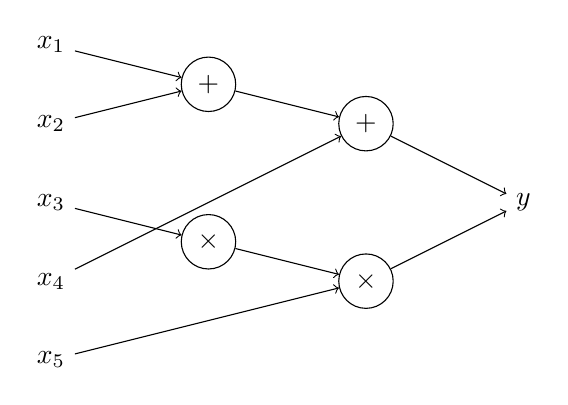
\begin{tikzpicture}
    % Nodes
    \node (input1) at (0, 4) {$x_1$};
    \node (input2) at (0, 3) {$x_2$};
    \node (input3) at (0, 2) {$x_3$};
    \node (input4) at (0, 1) {$x_4$};
    \node (input5) at (0, 0) {$x_5$};
    
    % First layer of gates
    \node[draw, circle] (add1) at (2, 3.5) {$+$};
    \node[draw, circle] (mul1) at (2, 1.5) {$\times$};
    
    % Second layer of gates
    \node[draw, circle] (add2) at (4, 3) {$+$};
    \node[draw, circle] (mul2) at (4, 1) {$\times$};
    
    % Output
    \node (output) at (6, 2) {$y$};
    
    % Connections
    \draw[->] (input1) -- (add1);
    \draw[->] (input2) -- (add1);
    \draw[->] (input3) -- (mul1);
    
    \draw[->] (add1) -- (add2);
    \draw[->] (input4) -- (add2);
    
    \draw[->] (mul1) -- (mul2);
    \draw[->] (input5) -- (mul2);
    
    \draw[->] (add2) -- (output);
    \draw[->] (mul2) -- (output);
    
\end{tikzpicture}

\end{document}
